\chapter{Introduction}\label{chapter:introduction}

Cyber-physical systems (CPS) and the Internet of Things (IoT) are rapidly accelerating the pace of evolution in the production of embedded systems. Spanning the range of personal devices for recreation and comfort, critical-care medical implants and monitors, intelligent transportation systems, and large-scale industrial facilities, embedded systems underlie the fabric of modern society and are commonplace in nearly all aspects of human daily activities. The benefits of widespread adoption include advances in financial management, health and welfare, economic output and productivity, and recreation. By and large, these benefits derive from distributed physical environment sensing and actuation integrated with data analytics. %CPS involves the integration of computing (i.e., embedded devices), physical systems (i.e., humans in the loop), and networking components in a unified scheme while being controlled by a computing system. CPS has applications in smart home, connected vehicles, industrial automation, power grids, aircraft system, medical devices, and buildings~\cite{Rajkumar:2010:CSN:1837274.1837461}. \textcolor{blue}{As a result of advancements in CPS research, we are able to control home devices remotely~\cite{Kadima, DeRussis}, communicate surrounding information from one vehicle to another in real-time~\cite{5454256, DBLP:journals/corr/abs-1304-3357}, perform automated at home monitoring and control of chronic diseases~\cite{6197404,doi:10.1155/2014/217415}. The progression in development and deployment of CPS can be attributed to the advancement in networking and embedded systems technology. CPS mainly comprises of embedded systems which are the building block to its computational component. Embedded systems are focused on computation and less on the interactions with the physical environment.}
%
Ubiquitous deployment of embedded systems with access to Internet gateways has led to the exponential growth of the IoT, which consists of heterogeneous, multiscale CPSs. Unfortunately, the rapid connection of these systems to external networks increases their attack surface and remotely exploitable vulnerabilities introduce new attack vectors that can have disastrous financial and physical impacts. In 2010 Stuxnet~\cite{stuxnet}---a sophisticated self-replicating virus---was discovered that successfully exploited vulnerabilities in industrial control system (ICS) software. In 2015, security researchers demonstrated a remote exploit targeting a Jeep vehicle that allowed the attacker to completely control the compromised automobile over the Internet~\cite{jeep_vulnerability}. In 2016, an exploitable vulnerability was discovered that enabled Internet-connected smart thermostats to be attacked by remote ransomware~\cite{smart_thermostat}. Such exploits can have devastating and long-lasting impact on individuals, institutions, and even nation-states.

\par A major security challenge for CPSs is ensuring trust in data. Data are trustworthy in case malicious agents have not tampered with the source or transformation of the data. A means of ensuring such trust is through data provenance, which identifies both the origin of data and their lineage through the history of data transformation. The record of provenance reveals intricate dependencies among data objects that enables auditing their production and use. Thus, data provenance addresses a key component of Lampson's ``gold standard'' of security~\cite{lampson_computer_2004}.  As a tool for security, data provenance is used in forensic analysis~\cite{Xie_yulani, LI2014259} and intrusion detection systems (IDS)~\cite{Fadolalkarim, Yoon}. The inherent difficulty in provenance collection is managing the growth of provenance, which increases each time a new data object is created or an existing one is manipulated; most important, even if one data object replaces another data object, the provenance records contain the source and lineage information about both. In systems with limited storage, such as embedded systems in a CPS, this difficulty is keen.

\par This dissertation introduces {\em Prov-CPS} as a framework for provenance collection in the kinds of resource-constrained embedded system devices found in fielded CPSs. Prov-CPS uses a streaming approach to achieve time-efficient generation of provenance, and prunes streaming provenance at the originating device for economic memory use. The construction of provenance is divided in two distinct phases by Prov-CPS: first, application source code is instrumented to generate traces of events relevant to an application's data use, and second the traces are converted to a provenance graph representation suitable for use in provenance analysis tools. This two-phase, trace-based approach is better suited to CPS software than prior provenance collection frameworks~\cite{hi_fi, muniswamy_reddy, 190900}, which collect provenance through operating system event monitoring (i.e., system calls and file accesses) that is impractical for resource-constrained embedded systems that often use baremetal software or a minimal real-time operating system without the necessary facilities or available computation and memory to implement such frameworks. Prov-CPS does not require an operating system. An ontological provenance data model~\cite{prov_dm} provides a unified semantic for representing provenance across heterogeneous devices and applications, which enables flexible mechanisms for application-defined control over both time and space resource utilization. We demonstrate and evaluate Prov-CPS using an anomaly-based IDS that analyzes provenance graphs. 

%\item  In designing a provenance-aware system, an application should utilize of a unified semantic for data model representation which fosters interoperability of heterogeneous devices captured. Unfortunately, most provenance data models \cite{6624109, 10.1007/11516798_9, olufowobi2016data, sabine_provenance} are not developed to model provenance data in a generic fashion. 

%\section{Provenance-Aware IoT Device Use Case}
%
%\begin{figure}[tb]
%\begin{center}
%%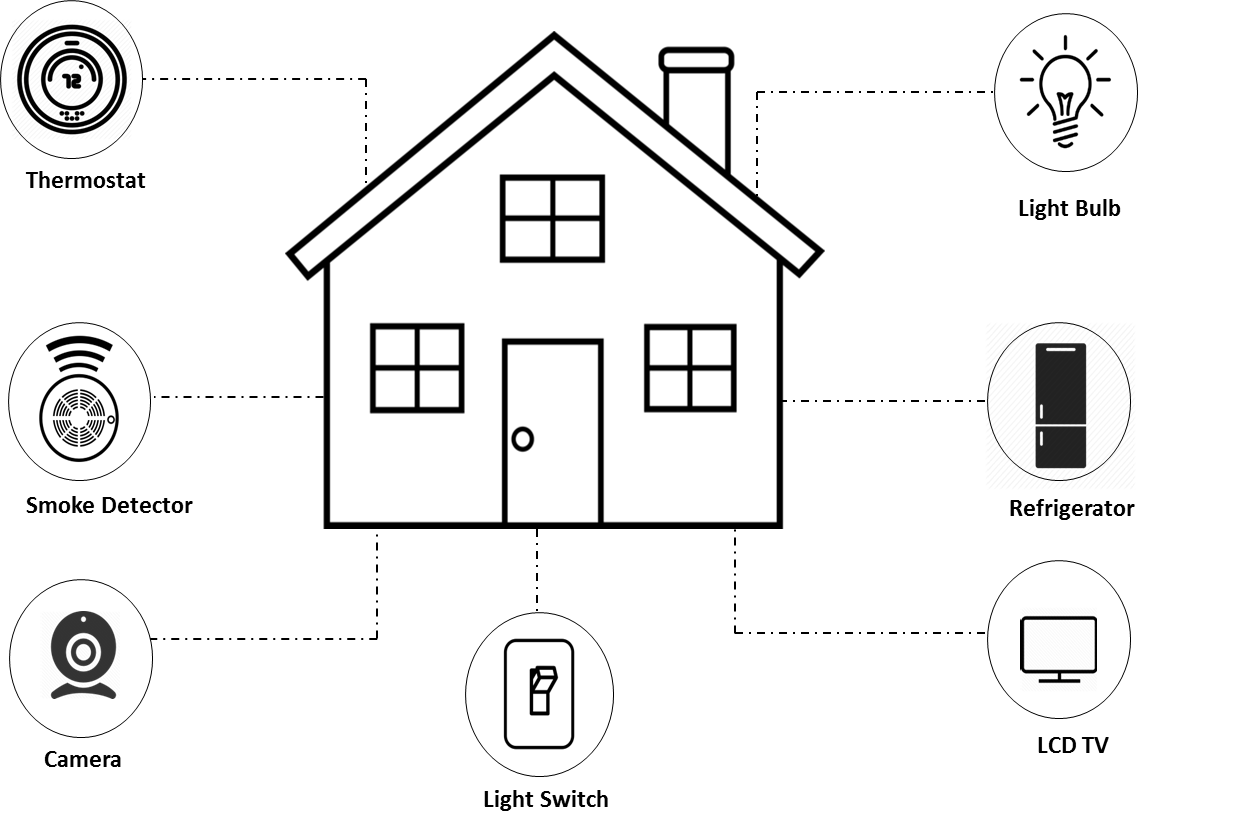
\includegraphics[height=3in]{smart_home_use_case.png}
%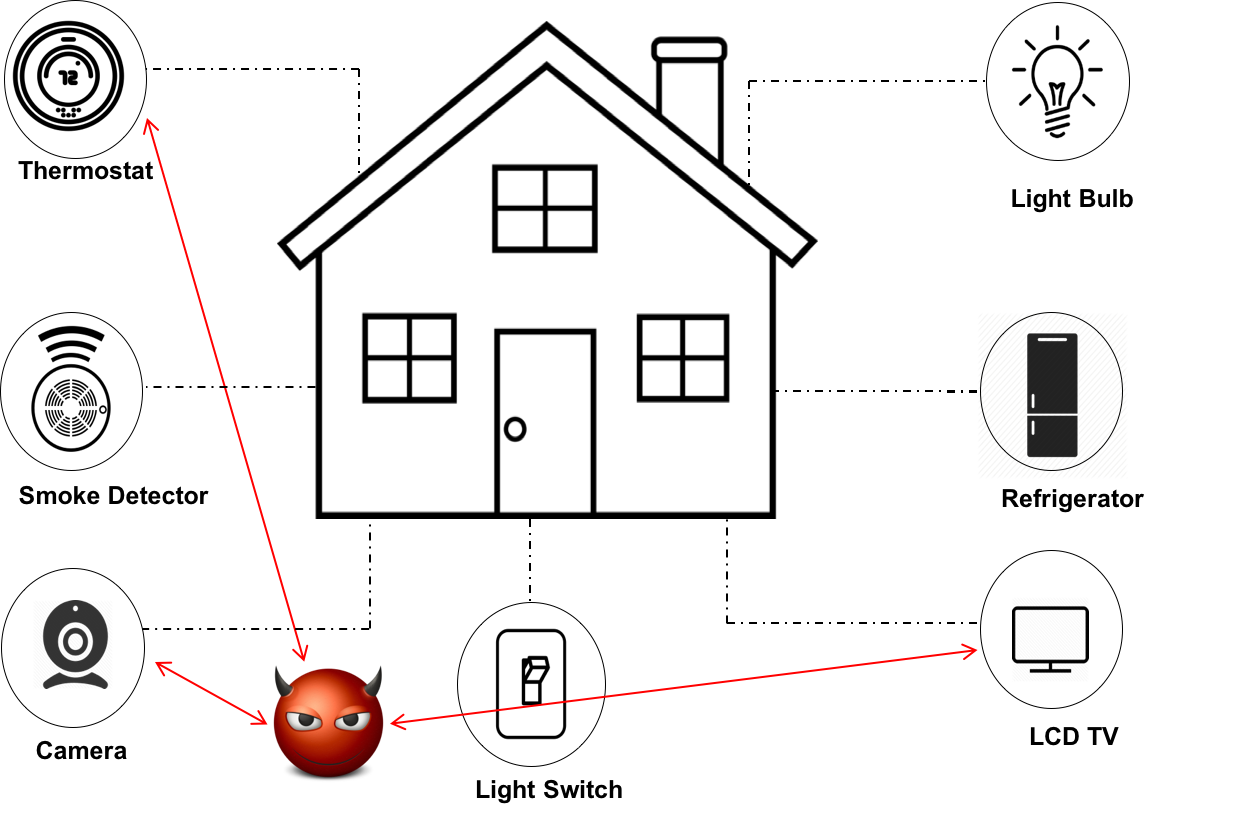
\includegraphics[height=4in]{smart_home_2.png}
%\end{center}
%\caption{Smart home use case Diagram}
%\label{smart_home}
%\end{figure}



%Consider a smart home as illustrated in Figure \ref{smart_home} that contains interconnected devices such as a thermostat which automatically detects and regulates the temperature of a room based on prior information of a user's temperature preferences, a smart lock system that can be controlled remotely and informs a user via short messaging when the door has been opened or is closed, a home security camera monitoring system, a smart fridge which sends a reminder when food products are low. In an event that a malicious intruder attempts  to gain access to the smart lock system and security camera remotely, provenance information can be used to track the series  of events to determine where and how a malicious attack originated. Provenance can also be used as a safeguard to alert of a possible remote or insider compromise thereby protecting against future or ongoing malicious attacks. 





%\section{Research Questions}
%The unification of data provenance and CPS and IoT is essential to the security of data disseminated. However, the unification raises some important research issues some of which are as a result of pre-existing provenance and IoT related issues. Some of the issues raised as a result of the unification of data provenance with IoT are outlined below:
%
%\begin{itemize}
%
%\item \textbf{Modeling provenance data:} How do we model provenance data collected from sensors and actuators contained in IoT architecture? Are there models used to represent causality between sensor and actuator readings in the IoT architecture.
%
%\item \textbf{Memory constraints on IoT Devices:} The vast amounts of data generated leads to high storage space utilization. Memory and data management techniques should be employed for efficient storage of provenance data on memory constrained devices. How do we effectively collect provenance data in resource constrained devices and relate this information across layers of the IoT architecture
%
%
%
%\item \textbf{Provenance data application utilization:} How do we utilize provenance data generated by provenance collection system to provide intrusion detection or digital forensics.
%
%
%
%\end{itemize}

\section{Research Contribution}

This dissertation makes the following contributions:


\begin{itemize}

\item \textbf{Prov-CPS: trace-based provenance collection framework.} The design and implementation of a provenance collection framework for capturing trace-based events for tracking data flow in an application's logic. This framework generates a trace of streaming events through application instrumentation with low execution run-time overhead that is decoupled from the more resource-intensive activities of provenance processing and analysis.

\item \textbf{Provenance data model for trace events.} A unified data model that represents the information flow semantics of data movement among components in an abstract CPS. This abstraction is mapped to real CPSs to facilitate automation of provenance data collection and analysis.

\item \textbf{Storage optimization through trace event pruning.} Support within the Prov-CPS framework for data pruning algorithms that discard events from streaming trace data prior to their conversion to provenance. These algorithms can be tailored to the needs of the provenance analyst yet take advantage of application domain knowledge.

\item \textbf{Experimental evaluation of Prov-CPS.} Prov-CPS is evaluated using an IDS applied to a climate control system data. Additionally, evaluation of the efficiency of Prov-CPS in space, with and without pruning, using a provenance-based IDS that identifies anomalies in data provenance records.



\end{itemize}

\section{Organization of Dissertation}

The remaining portion of this dissertation is organized as follows: In chapter 2, we review background information on CPS, IoT, Anomaly detection, and data provenance. We also discusses PROV-DM, a model for representing provenance. In Chapter 3, we outline related work on provenance collection systems, provenance-based pruning techniques, and provenance-based intrusion detection techniques. In Chapter 4, we give a detailed description of Prov-CPS, and provenance-trace data model. In Chapter 5, we describe our pruning heuristics. In Chapter 6, we discuss our anomaly detection algorithm using provenance graphs. Finally, we conclude in Chapter 7 with future research directions.

